% !TEX TS-program = pdflatex
% !TEX encoding = UTF-8 Unicode

% This is a simple template for a LaTeX document using the "article" class.
% See "book", "report", "letter" for other types of document.

\documentclass[11pt]{article} % use larger type; default would be 10pt

\usepackage[utf8]{inputenc} % set input encoding (not needed with XeLaTeX)
\usepackage{amsmath}
\usepackage{url}

%%% Examples of Article customizations
% These packages are optional, depending whether you want the features they provide.
% See the LaTeX Companion or other references for full information.

%%% PAGE DIMENSIONS
\usepackage{geometry} % to change the page dimensions
\geometry{a4paper} % or letterpaper (US) or a5paper or....
% \geometry{margins=2in} % for example, change the margins to 2 inches all round
% \geometry{landscape} % set up the page for landscape
%   read geometry.pdf for detailed page layout information

\usepackage{graphicx} % support the \includegraphics command and options

% \usepackage[parfill]{parskip} % Activate to begin paragraphs with an empty line rather than an indent

%%% PACKAGES
\usepackage{booktabs} % for much better looking tables
\usepackage{array} % for better arrays (eg matrices) in maths
\usepackage{paralist} % very flexible & customisable lists (eg. enumerate/itemize, etc.)
\usepackage{verbatim} % adds environment for commenting out blocks of text & for better verbatim
\usepackage{subfig} % make it possible to include more than one captioned figure/table in a single float
% These packages are all incorporated in the memoir class to one degree or another...

%%% HEADERS & FOOTERS
\usepackage{fancyhdr} % This should be set AFTER setting up the page geometry
\pagestyle{fancy} % options: empty , plain , fancy
\renewcommand{\headrulewidth}{0pt} % customise the layout...
\lhead{}\chead{}\rhead{}
\lfoot{}\cfoot{\thepage}\rfoot{}

%%% SECTION TITLE APPEARANCE
\usepackage{sectsty}
\allsectionsfont{\sffamily\mdseries\upshape} % (See the fntguide.pdf for font help)
% (This matches ConTeXt defaults)

%%% ToC (table of contents) APPEARANCE
\usepackage[nottoc,notlof,notlot]{tocbibind} % Put the bibliography in the ToC
\usepackage[titles,subfigure]{tocloft} % Alter the style of the Table of Contents
\renewcommand{\cftsecfont}{\rmfamily\mdseries\upshape}
\renewcommand{\cftsecpagefont}{\rmfamily\mdseries\upshape} % No bold!

%%% END Article customizations

%%% The "real" document content comes below...

\title{1-D Schrodinger's Equation Numerical Solution}
\author{Steve Clark}
%\date{} % Activate to display a given date or no date (if empty),
         % otherwise the current date is printed 

\begin{document}
\maketitle

\section{Introduction}
\par This project revolves mostly around the Time-Independent Schrodinger Equation(1-D) in Quantum Mechanics. The following is the full form of this equation:
\begin{equation}
E_n \psi _n (x) = \frac{-\hbar ^2}{2m}\nabla ^2 \psi _n (x) + V(x) \psi_n(x)
\end{equation}
\par This ultimately amounts to an Eigenvalue equation where $E_n$ are the energy eigenvalues, $\psi _n$ are the stationary state wavefunctions, and $V(x)$ is the potential function that the particle is interacting with. The reason this is time-independent is because these are what's known as stationary states, meaning any particle in one of these states will remain in this state for all future times. This is a very interesting consequence of these wave-functions, as it leads to some very intriguing results regarding energy measurements for quantum mechanic particles. This will be discussed further later in the text. 
\par The operator $\frac{-\hbar ^2}{2m}\nabla ^2$ is the kinetic energy of the particle, and the $V(x)$, as mentioned before, is the potential the particle interacts with. From classical physics, we can combine these into what is known as the "Hamiltonian" operator, commonly reffered to simply as $\hat{H}$. Since we can determine that the Hamiltonian operator is related to a physically observable phenomenon, we are allowed to conclude that the Matrix must be Hermitian, and therefore possesses only real eigenvalues. These eigenvalues are the discretized energy levels for the potential function $V(x)$. 
\par The Hamiltonian operator exists in an infinite-dimensional mathematical construct known as a Hilbert Space. The basis vectors in this space are the $\psi _n$ functions described earlier. While these are functions, they really correspond to eigenvectors of this Hamiltonian matrix. The other amazing thing about these stationary states is that since these $\psi _n$ functions are eigenvectors, they can be used as a set of linealy independent vectors that span the Hilbert Space. What this essentially means is that if one can find all of these stationary state wavefunctions, they can express any possible wavefunction for that specific Hamiltonian as a linear superposition of these basis vectors. This even includes wavefunctions that are not independent of time. 
\par The goal of this project is to find these stationary state wavefunctions for potentials that one can not analytically determine. Since these potentials bring with them a much more complicated set of differential equations, it becomes almost impossible to solve these eigenvalue problems for any sort of non-trivial potentials. That is why these must be solved numerically. 
\subsection{Some Simple Analytical Examples}
\subsubsection{Particle-In-A-Box}
As mentioned before, it becomes very difficult to solve these problems for complicated potentials, but there are a few potentials that we can solve analytically. These will provide a fundamental grounding that will allow the numerical algorithms' solutions to be compared with their analytical results. The first one we will look at is the infamous "Particle in a box" or "Infinite Square Well" potential. This potentially is given by the following:
\begin{equation}
V(x) =
\begin{cases}
0 & \text{if $0 < x < a$} \\
\infty & \text{otherwise}
\end{cases}
\end{equation}
Since the potential inside the box is $0$, it makes the problem into a fairly simple second-order differential equation:
\begin{equation}
\frac{-\hbar ^2}{2m}\frac{d^2}{dx^2}\psi _n = E\psi _n
\end{equation}
It is important to know that there is a time-dependent portion for this wavefunction, but for this project, only the spatial wave-functions will be examined. The time-dependence of a wave-function is actually quite trivial, once the stationary states have been found. 
\par Solving this equation, we obtain the following:
\begin{equation}
\psi _n = A_n sin(k_nx)
\end{equation}
\begin{equation}
k_n = \frac{n\pi}{a}
\end{equation}
We will look at the $A_n$ in more detail later in the next section. 
\par The value $n$ is simply an integer, so starting with $n=0, 1, 2, 3...$ we have determined all stationary state wavefunctions for the particle-in-a-box. Since the potential is $\infty$ on the outer edge of the box, we have the boundary condition that the wave-functions must vanish at the endpoints, and in fact these do, so we have proven that these solutions do satisfy the necessary conditions of the potential.  What about the associated energy eigenvalues? We have that:
\begin{equation}
E_n = \hbar \omega = \frac{\hbar ^2 k_n^2}{2m}
\end{equation}

\subsubsection{Harmonic Oscillator}
The Infinite-Square-Well Potential is one that is easy enough for us to analytically determine, because it really is a very simple differential equation. One that is slightly more complicated however, is the Harmonic Potential Oscillator. The potential function for aa Harmonic Oscillator is given by:
\begin{equation}
V(x) = \frac{1}{2}kx^2
\end{equation}
We can solve this problem, but in a slightly different way than what we used to solve the previous problem. Without going into too much detail, we use a construct called "Ladder Operators". These operators, unlike $\hat{H}$ are NOT Hermitian. An interesting property of these operators is that they are constructed in such a way that $\hat{a_-}\psi_n = \psi_{n-1}$ and $\hat{a_+}\psi_n = \psi_{n+1}$  Using these operators, it is quite simple prove that the Harmonic Oscillator has Energy Eigenvalues given by:
\begin{equation}
E_n = (n+\frac{1}{2})\hbar \omega
\end{equation}
(See \cite{BU} for full derivation)
\\
\par The wavefunctions themselves are relatively complex to write out in analytical form, but they all have the following form:
\begin{equation}
\psi _n(x) = A_n e^{-x^2} H_n(x)
\end{equation}
where $H_n$ are the so-called "Hermite Polynomials". It's fairly easy to see that even for quite a simple potential function, the solutions are already becoming extraordinarily complex. This is where it becomes necessary to solve these problems numerically.
\section{Numerical Algorithm}
\subsection{Finite Difference}
The first method presented here is the Finite Difference Method. This is a very straight forward algorithm that uses a finite forward-step in order to determine the next point using the previous two, as well as the finite definition for second derivative. This is not a very excellent method in terms of error, but it is by far the simplest to program. It is capable of solving second-order boundary-value differential equations quickly and without the need to decompose into sets of first-order equations. The exact equation used to determine the finite step is given by the following:
\begin{equation}
\psi _{n+1} = 2\psi _n - \psi _ {n-1} -2 (\Delta x)^2(E - V(x))
\end{equation}
where $E$ is the associated energy eigenvalue for the wavefunction, and V(x) is the potential at the point associated with the location of $\psi _n$. This can easily be used to plot wave-functions, if the energy eigenvalues are known. 
\par This first run of the program is for the Infinite Square Well potential. It uses an algorithm(which will be discussed later) to compute the energy eigenvalues, and then plots the waveforms via the finite-difference method explained above. The results are shown in Figure 1 below.
\par Returning to the $A_n$ value from before, these wavefunctions have the following necessary property:
\begin{equation}
\int_{-\infty}^\infty|\psi |^2 = 1
\end{equation}
because the wavefunctions are deemed as being Normalizable. The quantity $|\psi |^2$ is actually the probability density for the wavefunction. This gives the probability that a function will be located at a certain position as a function of the spatial coordinate $x$. If one integrates all of these finite probabilities over all space, the total probability must be exactly 1, because the particle must exist somewhere. Due to this condition, we can solve for the $A_n$ values. The analytical result gives $A_n = \sqrt{\frac{2}{a}}$. Since this is a numerical simulation however, a simple rectangular Riemann Sum for $N = 1000$ was used to determine this coefficient. 
\begin{figure}
\centering
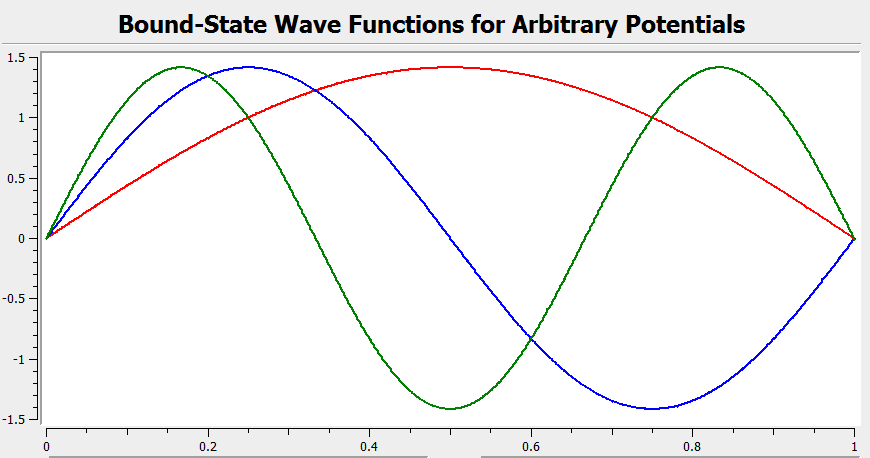
\includegraphics[scale = .5]{fp1}
\caption{First Three Eigenstates for Infinite Square Well}
\end{figure}
\par Since we are assuming $a = 1$, the determined value for this constant should be about $\approx 1.4$, and indeed this is the case as shown in Figure 1.  To get some idea of just how accurate these functions are, the residuals between the numerical results and the analytical results are plotted in Figure 2. The error is most often on the order of $10^{-4}$, so these are definitely accurate solutions. 
\begin{figure}
\centering
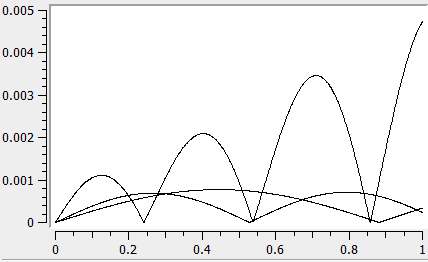
\includegraphics{fp2}
\caption{Residuals for Infinite Square Well as a function of x}
\end{figure}
\subsection{Finding Energy Eigenvalues}
The real complication for this project arises in finding the energy eigenvalues. The Finite Difference Algorithm has clearly shown its effectiveness for accurate input energies, but finding these energies can be tricky. The Infinite Square Well potential is a fairly simple one to solve because we know that the wavefunction vanishes entirely at the end points of the well. However, most potential functions do not have this luxury. Rather, they meet the boundary condition that $\psi (\pm \infty) = 0$. Numerically, this means we must choose a finite interval for $x$ and say that the wave-function vanishes at its endpoints. This will unfortunately introduce some error because it's not technically true. In the classically forbidden regions, the wavefunction drops off exponentially, so as long as we can extend these conditions far enough, we can assume that the wavefunction will be approximately zero.
\subsubsection{Shooting Method}
The method described here is aptly named the "Shooting Method". It is not very resource efficient, and it takes quite a bit of time computationally, but it's a very simple to program and accurate method for determining energy eigenvalues. 
\par Using the boundary conditions described earlier, we must find which values of energy satisfy them as accurately as possible. We determine this by using a modified bisection method. Simply figure out all of the possible values for $\psi (x_{max})$ as a function of energy, and find where it occurs that this value changes sign. Via the Intermediate Value Theorem, we can conclude that a zero must exist in between these two values of energy. I have a function called "findE" that will test create a 50 point array of energies between these two values and test all of them for an input tolerance value. If it does not find any $E$ values that fall below this tolerance level, it will recursively call itself with the two values in this new array such that $\psi (x_{max})$ changes sign.  Once it has reached a value below this tolerance, it will return the energy value as an eigenvalue. Figure 3 below shows why this algorithm works. If the value of the energy is off even by a little bit, the necessary boundary conditions will not be met, and therefore it could not possibly be a solution to the Time-Independent Schrodinger Equation. 
\begin{figure}
\centering
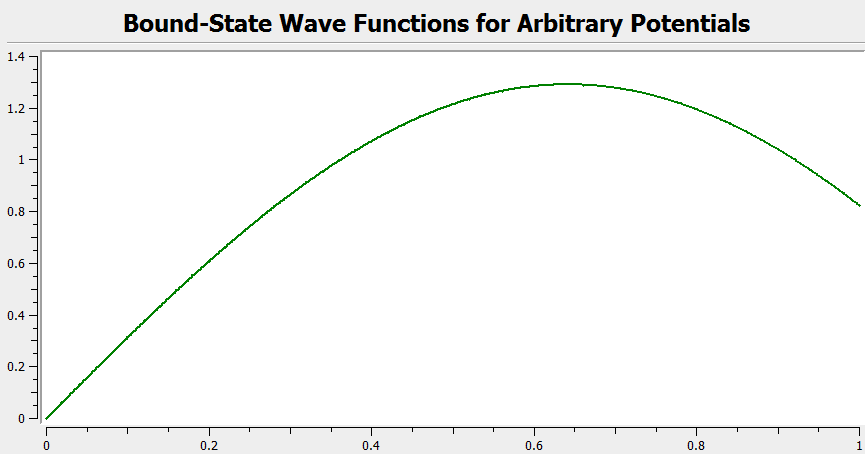
\includegraphics[scale = .5]{fp3}
\caption{Energy = 3.0 (Not an eigenvalue)}
\end{figure}
In order to determine how accurate this algorithm is, we will again refer to the analytical results for the Infinite Square Well and Harmonic Oscillator Potentials.  Figure 4 shows the numerically determined energy values and the $\log _{10} (error)$. 
\begin{figure}
\centering
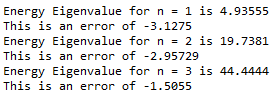
\includegraphics{fp4}
\caption{Eigenvalues for Infinite Square Well}
\end{figure}
\par Figures 5 and 6 show the wavefunctions and energy eigenvalues for the harmonic oscillator potential. 
\begin{figure}
\centering
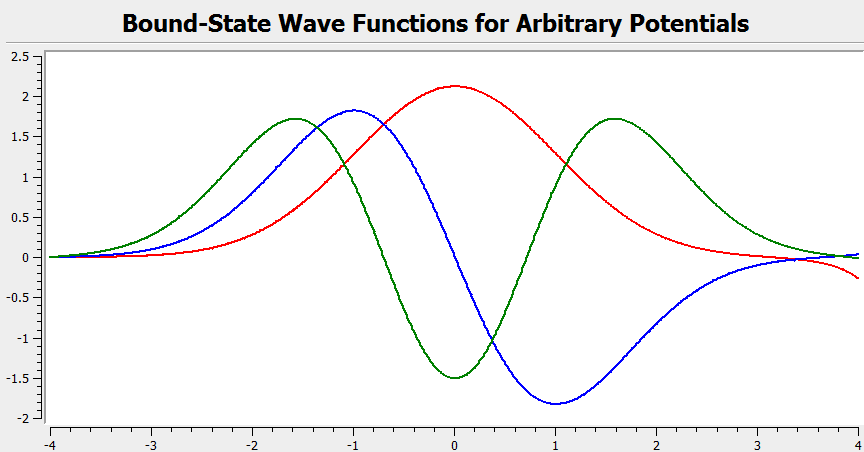
\includegraphics[scale = .5]{fp5}
\caption{Wavefunctions for Harmonic Oscillator Potential}
\end{figure}
\begin{figure}
\centering
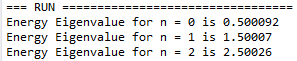
\includegraphics{fp6}
\caption{Energy Eigenvalues for Harmonic Oscillator}
\end{figure}
\par For the numerical simulation, we have that $\hbar = \omega = 1$, so our values should simply be $E_n = n + \frac{1}{2}$, and indeed these are very close to the results we obtain. Another interesting thing to note is in Figure 5. It becomes clear that the integration is unstable in the classically forbidden region. This makes the task of having one program for an arbitrary input potential very difficult. I've found that occasionally I would have to change certain parameters inside the program around to make it work better, so not just the user-input values are always enough. I could add more values to the front panel, but I think it's just easier to manipulate it from inside the program itself. 
\section{Results}
Now that we have seen the effectiveness of these algorithms, this section will present some more complicated results and analysis. 
\par The first potential to look at will be the anharmonic oscillator. This potential is given by:
\begin{equation}
V(x) = \frac{1}{2}x^2 + x^4
\end{equation} 
The first part of the potential is just the harmonic oscillator we're used to, by the $x^4$ term is what makes this an anharmonic oscillator instead. To those running this code, it does take a bit of time to do all of the calculation. This calculation took on the order of 2 or so minutes to complete. It should also be mentioned that for this code, I change the x-array in the "findE" function to be between -1.5 and 1.5 instead of what it was for the Harmonic Oscillator $\pm 4$.  It's important to note that the wavefunctions are sensitive to these conditions, as mentioned earlier. Since the potential is growing like $x^4$ though, one can sufficiently say that these bounday conditions are realistic even for $x = 1.5$.  Figures 7 and 8 show the outputs for this potential. The wavefunctions themselves look very similar, which makes sense considering it's an entirely even potential, but the energies are much higher than for the harmonic oscillator. This also makes sense, looking at the Time-Independent Schrodinger equation because the potentials are growing much more quickly. 
\begin{figure}
\centering
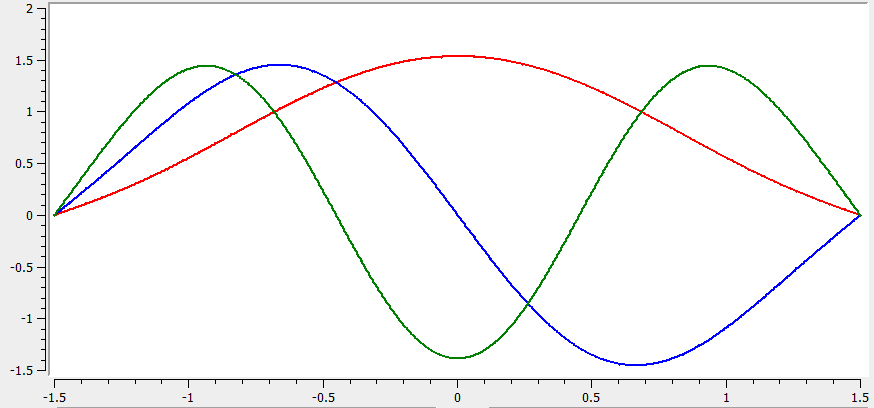
\includegraphics[scale = .5]{fp7}
\caption{Wavefunctions for Anarmonic Oscillator Potential}
\end{figure}
\begin{figure}
\centering
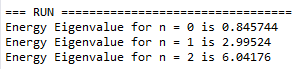
\includegraphics{fp8}
\caption{Energy Eigenvalues for Anharmonic Oscillator}
\end{figure}
\par The final potential I'd like to look at is referred to as the "Morse Potential". It has the following form:
\begin{equation}
V(x) = (1 - e^{-x})^2
\end{equation}
Since this potential is much more complicated, I have also included with the normal plots, a plot of the Morse Potential. Since it only shows a piece of the graph from $x=-.5$ to $x =4$, I will also mention that it diverges to infinity for negative x, and it approaches $1$ asymptotically in the limit as $x \to \infty$. 
\begin{figure}
\centering
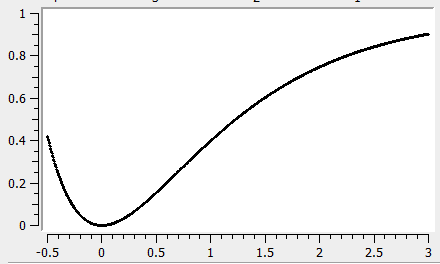
\includegraphics{fp9}
\caption{Morse Potential}
\end{figure}
\begin{figure}
\centering
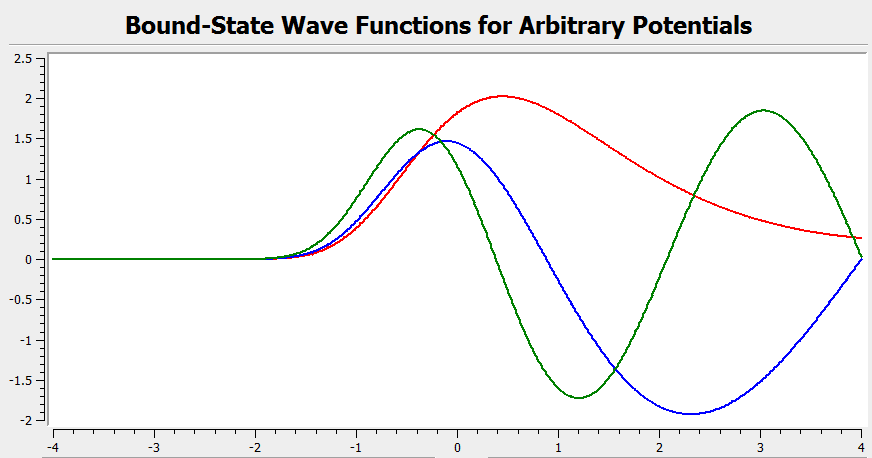
\includegraphics[scale = .5]{fp10}
\caption{Morse Potential Stationary State Wavefunctions}
\end{figure}
\begin{figure}
\centering
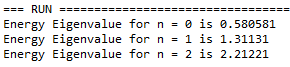
\includegraphics{fp11}
\caption{Morse Potential Energy Eigenvalus}
\end{figure}
\begin{thebibliography}{9}

\bibitem{UCT}
\url{http://www.phy.uct.ac.za/courses/opencontent/phylab2/worksheet4_09.pdf}
\bibitem{emory}
\url{http://www.chemistry.emory.edu/faculty/bowman/old_classes/chem430sp99/num%20sol/NUM%20SOL.html}
\bibitem{BU}
\url{http://physics.bu.edu/~py502/lectures4/schrod.pdf}
\bibitem{wiki}
\url{http://www.en.wikipedia.org}
\end{thebibliography}


\end{document}
